\chapter{Random Graph Ensembles}

In this chapter, we will explore the concept of random graph ensembles, which are fundamental in understanding the properties and behaviors of complex networks. We will start with the simplest model, the Erdős-Rényi random graph, and then move on to more complex models such as the Stochastic Block Model (SBM). We will also discuss the thermodynamic limit, degree distribution, phase transitions, and other properties of these random graph ensembles.

\section{Erdős-Rényi Random Graphs}

We are going to start with the simplest model of random graphs, which is the Erdős-Rényi (E-R) model. This model serves as a fundamental null model for understanding the properties of complex networks.

\begin{definition}[Erdős-Rényi Random Graphs]
    Networks whose interactions (links) between nodes are chosen randomly, without a priori correlations or rules. In statistical mechanics terms, it is comparable to a ``perfect gas'' with molecules (nodes) experiencing random ``sparse'' impacts (links).
\end{definition}
It can be seen as a \textbf{null model} for complex networks, as it represents a system with no structure or correlations, and it can be used as a baseline for understanding real-world networks.

If we expect to find a certain property in a real network, we can compare it to the expected value of that property in an E-R random graph. If the observed value significantly deviates from the expected value, we can infer that there is some underlying structure or correlation in the real network that is not captured by the E-R model. It can also be used to confront different systems, such as comparing the structure of a social network to that of a biological network, to identify unique features and commonalities.

If we make the statistical analogy with a gas, the E-R model represents a perfect gas, where the nodes are like molecules that interact randomly without any specific rules or correlations. The edges, which are generated randomly, represent some average quantities of the system, not the distance between nodes or the strength of interactions. The E-R model is a useful starting point for understanding the properties of complex networks, but it is important to note that real-world networks often exhibit more complex structures and correlations that are not captured by this simple model.

\section{Statistical Ensembles of Networks}

If we imagine to take a picture of our ideal gas system, we would see a random distribution of molecules (nodes) and their interactions (links, diluted interactions, since we are speaking of ideal gas). The E-R model captures this randomness and serves as a baseline for understanding the properties of complex networks. In the next instant, the picture would change, and we would see a different random distribution of molecules and interactions, but the overall properties of the system would remain the same, as they are determined by the average quantities rather than the specific configuration of nodes and links. We will see that these analogies with ensambles will be very useful to understand the properties of complex networks, and also the E-R model will mantain some properties constant even if we change the specific configuration of nodes and links, which is a key feature of random graph ensembles.

We are going to use \textbf{ensembles of networks} with fixed parameters: same macroscopic state (e.g. link density, degree pdf) different microstates (single-node properties), and we will see that the properties of the ensemble are determined by the average quantities rather than the specific configuration of nodes and links.
The definition of the ensamble will suggest a construction rule to generate the microstates of the ensemble and to compute the probability of generating a specific microstate.

\begin{remark}
    The number of ALL symmetric networks (microstates) with N nodes (whatever the links) is:
    \[
        2^{\frac{N(N-1)}{2}}, \quad \sum_{i=1}^{N} \binom{N}{i} = 2^N.
    \]
    This means that the number of possible configurations of links between N nodes is exponential in the number of nodes, which highlights the complexity of the space of possible networks and the importance of using ensembles to understand their properties.
\end{remark}

The most common ensembles are the microcanonical ensemble, where we fix the number of links, and the canonical ensemble, where we fix the probability of having a link between two nodes. Let us introduce these two ensembles in more detail.

\subsection{Microcanonical Ensemble $G_{N,M}$}

\begin{definition}[Microcanonical Ensemble]
    An ensemble of networks with $N$ nodes, representing a fixed system size, and $M$ links, representing the system energy. The links are randomly selected from the possible $N(N-1)/2$ for a symmetric network or $N(N-1)$ for a direct graph.
\end{definition}

The idea behind a microcanonical ensemble is that we are looking at all possible configurations of a network with a fixed number of nodes and links. Each configuration (or microstate) is equally likely, and the properties of the ensemble are determined by the average quantities rather than the specific configuration of nodes and links.

Looking at the properties of the microcanonical ensemble, we can see that it is a very simple model, but it can still capture some important properties:
\begin{itemize}
    \item The \(N\) nodes represent the system size, which is fixed.
    \item The \(M\) links represent the system energy, which is also fixed.
    \item The links are randomly selected from the possible \(N(N-1)/2\) for a symmetric network or \(N(N-1)\) for a directed graph, which means that there is no specific structure or correlation in the network.
\end{itemize}
So we have
\[
    M_{max} = \frac{N(N-1)}{2}, \quad \# G_{N,M} = \binom{M_{max}}{M},
\]
such that for a fixed number of nodes \(N\) and links \(M\), the number of possible configurations (or microstates) of the network is given by the binomial coefficient \(\binom{M_{max}}{M}\), which counts the number of ways to choose \(M\) links from the total possible \(M_{max}\) links. This highlights the combinatorial nature of the microcanonical ensemble and the importance of using statistical methods to understand its properties.

\begin{remark}[Construction Rule]
    The construction rule of one instance of the ensemble is:
    \begin{enumerate}
        \item Take $N$ nodes.
        \item Repeat $M$ times: choose 2 nodes randomly and connect them, checking for loops or existing links.
    \end{enumerate}
    The probability of generating ``bad'' links, such as loops and multilinks, is about $1/N$. The effect of this selection becomes negligible for large $N$.
\end{remark}

The probability of generating a loop is $1/N^2$, and the probability of generating a multilink is $M/N^2$. In order to connect two times the same nodes, the probability is $1/N^2$. For large $N$, i.e. in the thermodynamic limit, these probabilities become negligible, and the microcanonical ensemble can be effectively generated by randomly selecting $M$ links from the possible $N(N-1)/2$ links without worrying about loops or multilinks.

Given the number of nodes \(N\) and links \(M\), the properties of the microcanonical ensemble are determined as well as the whole ensamble itself. Indeed with only those two parameters, we can build every possible configuration of the network, and we can compute the average properties of the ensemble, such as the degree distribution, clustering coefficient, and other network metrics.

\subsection{Canonical Ensemble $G_{N,P}$}

Often it is more convenient to \textbf{fix the probability} of having a link between two nodes, rather than the number of links. This leads us to the canonical ensemble.

\begin{definition}[Canonical Ensemble]
    An ensemble of networks with $N$ nodes (fixed system size) and a fixed probability $P$ to have a link between them, representing a fixed average energy or temperature of the system. The links are generated randomly with probability $P$ from the possible $N(N-1)/2$ for a symmetric network or $N(N-1)$ for a directed graph.
\end{definition}

This means that in the canonical ensemble, given the nodes and the probability $P$, we can generate a random graph by connecting each pair of nodes with a link with probability $P$. The properties of the ensemble are determined by the average quantities:
\[
    P = \langle E \rangle \propto T, \quad \langle l \rangle = P \frac{N(N-1)}{2}.
\]

\subsubsection{Binomial Link Distribution}

In the canonical ensemble, given a fixed number of nodes \( N \) and a connection probability \( P \), we do not have a fixed number of links. Instead, \textbf{ALL possible graphs} with \( N \) nodes mathematically belong to the ensemble \( G_{N,P} \), but each specific configuration occurs with a different probability depending on \( P \).

The probability \( p(m) \) of generating a graph with exactly \( m \) links and \( N \) nodes is governed by the binomial distribution:
\[
    p(m) = \binom{\binom{N}{2}}{m} \cdot P^m \cdot (1 - P)^{\binom{N}{2} - m}
\]
The expected (average) number of links in the entire network grows as:
\[
    \langle m \rangle = P \cdot \binom{N}{2} = P \cdot \frac{N(N-1)}{2}
\]
And the standard deviation of the number of links is given by:
\[
    \sigma_m = \sqrt{P \cdot (1 - P) \cdot \binom{N}{2}}
\]

\paragraph{Note: Node Degree Binomial (Bernoulli) Distribution}
If we shift our focus from the total links \( m \) to the specific degree \( k \) of a single node, this too is governed by a binomial probability density function. Assuming \( N \) independent trials (where connecting to each other node is a Bernoulli trial with success probability \( P \)):
\[
    p(k) = \binom{N}{k} \cdot P^k \cdot (1 - P)^{N-k} = \frac{N!}{k!(N - k)!} \cdot P^k \cdot (1 - P)^{N-k}
\]
\textit{(Note: strictly speaking, a node can connect to \( N-1 \) other nodes, but for large networks we approximate the number of trials to \( N \)).}

For a single node, the average degree is simply the expected value of \( N \) trials:
\[
    \langle k \rangle = \sum_k k \cdot p_k = P \cdot N
\]
The standard deviation of the node degree is \( \sigma = \sqrt{N \cdot P \cdot (1 - P)} \).

A crucial statistical property of this distribution is the \textbf{Coefficient of Variation (CV)}, which represents the relative error. As the network size \( N \) grows, the CV strictly tends to zero:
\[
    \frac{\sigma}{\langle k \rangle} \approx \frac{1}{\sqrt{N}} \xrightarrow{N \to \infty} 0
\]
This implies that in very large Erdős-Rényi networks, the degrees of almost all nodes tightly cluster around the average \( \langle k \rangle \), making the network strongly homogeneous.

\subsubsection{Algorithmic Construction Rules}

To computationally generate networks belonging to the \( G_{N,P} \) ensemble, we use the following stochastic rules based on the probability \( P \).

\textbf{Construction of an Undirected Graph:} the adjacency matrix \( A \) is symmetric, and we only need to consider the upper triangular part of the matrix (excluding the diagonal). The algorithm proceeds as follows:
\begin{enumerate}
    \item Take \( N(N-1)/2 \) values \( A_{ij} \) representing the upper triangular matrix (one value for each possible unique link). Distribute these values uniformly between 0 and 1.
    \item Apply the probability threshold: if \( A_{ij} > 1 - P \), then set \( A_{ij} = 1 \) (the link exists); else set \( A_{ij} = 0 \).
    \item Symmetrize the matrix to make the graph undirected using a logical "OR" operation: \( A \lor A^T \).
\end{enumerate}

\textbf{Construction of a Directed Graph:} the adjacency matrix \( A \) is not symmetric, and we need to consider all \( N(N-1) \) possible directed links (excluding self-loops). The algorithm proceeds as follows:
\begin{enumerate}
    \item Take \( N(N-1) \) values \( A_{ij} \), effectively covering the entire matrix but explicitly excluding the main diagonal (no self-loops). Distribute these uniformly between 0 and 1.
    \item Apply the exact same threshold: if \( A_{ij} > 1 - P \), then set \( A_{ij} = 1 \); else set \( A_{ij} = 0 \). (No symmetrization is applied).
\end{enumerate}

\paragraph{Thermodynamic Limit}
If the network is sufficiently large, the binomial degree distribution can be analytically approximated by a \textbf{Poisson distribution} (this occurs in the limit of large \( N \) and small \( P \), where the average degree \( \langle k \rangle = P \cdot N \) is kept constant).

This highlights the fact that in the canonical ensemble, while the exact number of links \( m \) can fluctuate widely depending on the specific stochastic realization, the macroscopic properties of the ensemble are predictably and strictly determined by the generation probability \( P \) and the number of nodes \( N \).

\subsection{Equivalence of Ensembles (Canonical to Microcanonical)}

In statistical mechanics, different ensembles often yield the same macroscopic behavior in the thermodynamic limit. This holds true for network ensembles as well.

For a large number of nodes (\( N \gg 1 \)), the variance of the binomial link distribution grows much slower than its mean. Consequently, the canonical link distribution becomes incredibly sharp, mathematically tending toward a \textbf{Dirac's delta function} centered exactly on the average value.

Because the probability collapses onto this single peak, \textbf{all instances} generated within the Canonical ensemble (\( G_{N,P} \)) will essentially have a fixed number of links equal to the expected average:
\[
    m \approx \langle m \rangle = P \frac{N(N-1)}{2}
\]
By converging to a state with a strictly fixed number of links, the canonical ensemble perfectly recovers the defining property of the \textbf{Microcanonical ensemble}.

\subsubsection{The "Balls and Holes" Analogy}
To intuitively understand the emergence of the binomial distribution, we can use the "balls and holes" analogy:
\begin{itemize}
    \item \textbf{Holes} represent the possible connections between nodes.
    \item \textbf{Balls (couples)} represent the actual edges being placed.
\end{itemize}
Imagine randomly dropping a finite number of balls into a set of discrete bins (holes). If you plot a histogram of how many balls land in each bin with finite sampling, the resulting shape is a \textbf{binomial probability density function (pdf)}. A perfectly flat, uniform pdf is only theoretically achieved in the infinite sampling limit.
\begin{figure}[H]
    \centering
    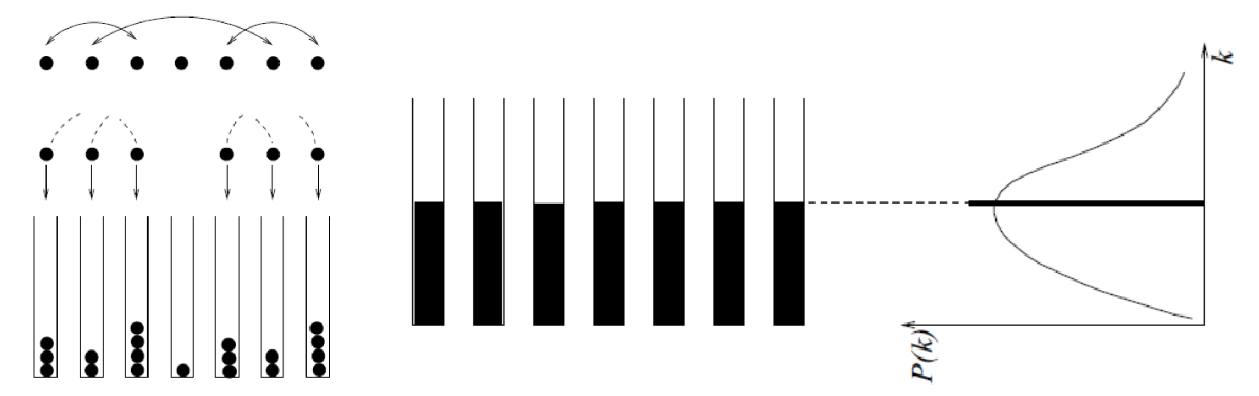
\includegraphics[width=0.8\textwidth]{img/balls_and_holes.png}
    \caption{The "Balls and Holes" analogy for understanding the binomial distribution in random graph ensembles.}
\end{figure}

\subsection{Degree Probability Density Function (pdf) in \( G_{N,P} \)}

Let us focus on the connectivity of a single node in a network of \( N \) nodes, where every possible link exists with independent probability \( P \).

The probability \( p(k) \) of a specific node having exactly \( k \) links (its degree) is equivalent to the probability of randomly succeeding exactly \( k \) times out of the \( N-1 \) possible trials (the other nodes). This is perfectly described by the Binomial distribution:
\[
    p(k) = \binom{N-1}{k} P^k (1-P)^{N-1-k}
\]

We can derive the \textbf{average node degree} \( \langle k \rangle \) by taking the total number of link-ends in the network (which is twice the average number of links) and dividing by the number of nodes \( N \):
\[
    \langle k \rangle = \frac{2 \cdot \langle \#\text{links} \rangle}{N} = \frac{2 \cdot P \frac{N(N-1)}{2}}{N} = P(N-1) \approx P \cdot N
\]
\textit{(Note: The average total link density of the network is simply \( P \frac{N(N-1)}{2} \)).}

\begin{remark}[The Thermodynamic Limit: Bernoulli \(\to\) Poisson \(\to\) Gauss \(\to\) Delta]
    As networks grow infinitely large, their statistical distributions undergo fascinating mathematical transformations.

    If we take the thermodynamic limit (\( N \to \infty \)) but force the network to remain sparse by scaling down the probability (\( P \to 0 \)) such that the average degree remains constant (\( P \cdot N = \lambda = \text{constant} \)), the Binomial (Bernoulli) distribution mathematically converges to a \textbf{Poisson distribution}:
    \[
        p(k) \approx \frac{\lambda^k}{k!} e^{-\lambda} \quad \text{where } \langle k \rangle = \lambda \text{ and } \sigma = \sqrt{\lambda}
    \]

    If we then look at highly dense networks where the constant \( \lambda \gg 1 \), the Poisson distribution further approximates to a \textbf{Gaussian (Normal) distribution}: \( \mathcal{N}(\lambda, \sqrt{\lambda}) \).

    Finally, as \( \lambda \to \infty \), the standard deviation becomes negligible compared to the mean, and the distribution collapses into a \textbf{Dirac Delta function}:
    \[
        \lim_{\lambda \gg 1} p(k) \to \delta(x - \lambda)
    \]
    \textbf{Physical Consequence:} In the absolute thermodynamic limit, a random Bernoulli graph behaves paradoxically like a \textbf{regular graph} where every single node has the exact same connectivity \( \lambda \). While it lacks the spatial ordered proximity of a crystal lattice, the Erdős-Rényi graph effectively acts as an \textbf{infinite-dimensional regular lattice} where all nodes are equally likely to be neighbors.
\end{remark}

\subsection{The Erdős-Rényi (E-R) Null Model and Phase Transitions}

Because of its pure randomness, the Erdős-Rényi network serves as the fundamental \textbf{null model} in complex network theory.

Its defining characteristics are:
\begin{itemize}
    \item \textbf{Absence of correlations:} There are no hidden structural biases, hierarchies, or correlations between node features (e.g., a node's degree does not influence the degree of its neighbors).
    \item \textbf{Single Macroscopic Parameter:} The entire topology of the ensemble is uniquely governed by one single macroscopic parameter: \( P \) (the probability of connection).
\end{itemize}

However, its simplicity hides complex thermodynamic behavior. A critical phenomenon of the E-R model is that \textbf{not all statistical properties vary smoothly} with the control parameter \( P \) as \( N \to \infty \).
By slowly increasing \( P \), the network can undergo sudden, abrupt \textbf{phase transitions}, the most famous being the spontaneous emergence of a "giant connected component" that suddenly bridges the majority of isolated nodes into a single macroscopic cluster at a specific critical threshold.








\section{Phase Transitions and the Giant Component}

When considering the probability of a specific property existing within a network ensemble of \(N\) nodes, we observe that this probability is a function of the network size:
\[
    P = P(N)
\]
Depending on the evolutionary trend of the network, we encounter behaviors that lead to certain topological properties being valid for \textit{almost all} graphs or \textit{almost none}. This abrupt shift is the hallmark of a \textbf{phase transition}—a critical threshold that sharply separates two radically different macroscopic states of the system.

In random graphs, the most significant phase transition is the sudden emergence of a \textbf{Giant Component (GC)}: a single, massive connected cluster that encompasses a macroscopic fraction of the entire network's nodes.

\subsection{Control Parameter: Average Connectivity}
In Erdős-Rényi (E-R) networks, the threshold for these topological transitions heavily depends on the network size \(N\) and the connection probability \(p\). To standardise this, we define the \textbf{average connectivity} \(\lambda\) as our primary control parameter:
\[
    \langle k \rangle \approx pN = \lambda
\]

\subsection{Emergence of the Giant Component}

\begin{definition}[Giant Component Regimes]
    \begin{itemize}
        \item For \(\lambda < 1\): There is \textbf{no giant component}. The network consists of isolated nodes and very small, fragmented clusters.
        \item For \(\lambda \geq 1\): A giant component suddenly emerges. As \(\lambda\) continues to increase, this giant cluster rapidly grows, tending to absorb and include all the nodes in the system, resulting in a fully connected network.
    \end{itemize}
\end{definition}

\subsubsection{Derivation: The Transcendental Equation}
To mathematically prove the existence of this critical point, let us define \(u\) as the probability that a randomly chosen node does \textbf{not} belong to the giant component (\(p(\notin G_c) = u\)).

Logically, if a node does not belong to the GC, it strictly means that \textit{all of its first neighbors} must also not belong to the GC. Assuming a large network (\(N \gg 1\)), we can use the Poisson approximation for the degree distribution \(p_k\):
\[
    p(k) = p_k = e^{-\lambda} \frac{\lambda^k}{k!}
\]
The probability \(u\) can be expressed via an average field equation. For a node with \(k\) neighbors, the probability that \textit{none} of them are in the GC is \(u^k\). Averaging this over all possible degrees gives:
\[
    u = \langle u^k \rangle = \sum_{k=0}^{\infty} p_k u^k
\]
Substituting the Poisson distribution:
\[
    u = e^{-\lambda} \sum_{k=0}^{\infty} \frac{(\lambda \cdot u)^k}{k!}
\]
Recognizing the Taylor series expansion for the exponential function (\(\sum \frac{x^k}{k!} = e^x\)), we obtain the fundamental \textbf{transcendental equation}:
\[
    u = e^{\lambda(u-1)}
\]

\subsubsection{The Order Parameter \(S\)}
In statistical mechanics, phase transitions are described by an order parameter. Here, we define \(S\) as the \textbf{fraction of nodes belonging to the giant component}.
Since \(u\) is the fraction of nodes \textit{outside} the GC, we have \(S = 1 - u\).

Substituting this into our transcendental equation yields the implicit equation for the order parameter:
\[
    S = 1 - e^{-\lambda S}
\]
Analyzing this equation reveals the phase transition:
\begin{itemize}
    \item If \(\lambda < 1\), the only valid physical solution is \(S = 0\) (meaning \(p_{GC} = 0\)).
    \item If \(\lambda > 1\), a non-zero solution for \(S\) appears. For increasing \(\lambda\), the value of \(S\) exponentially approaches 1, meaning the GC tends to occupy the entire graph.
\end{itemize}

\begin{figure}[H]
    \begin{minipage}{0.35\textwidth}
        \caption{The plot represents the Order Parameter S as a function of average connectivity lambda. The graph shows S remaining at 0 until lambda=1, at which point it steeply curves upwards and asymptotically approaches S=1.}
    \end{minipage}
    \hfill
    \begin{minipage}{0.6\textwidth}
        \centering
        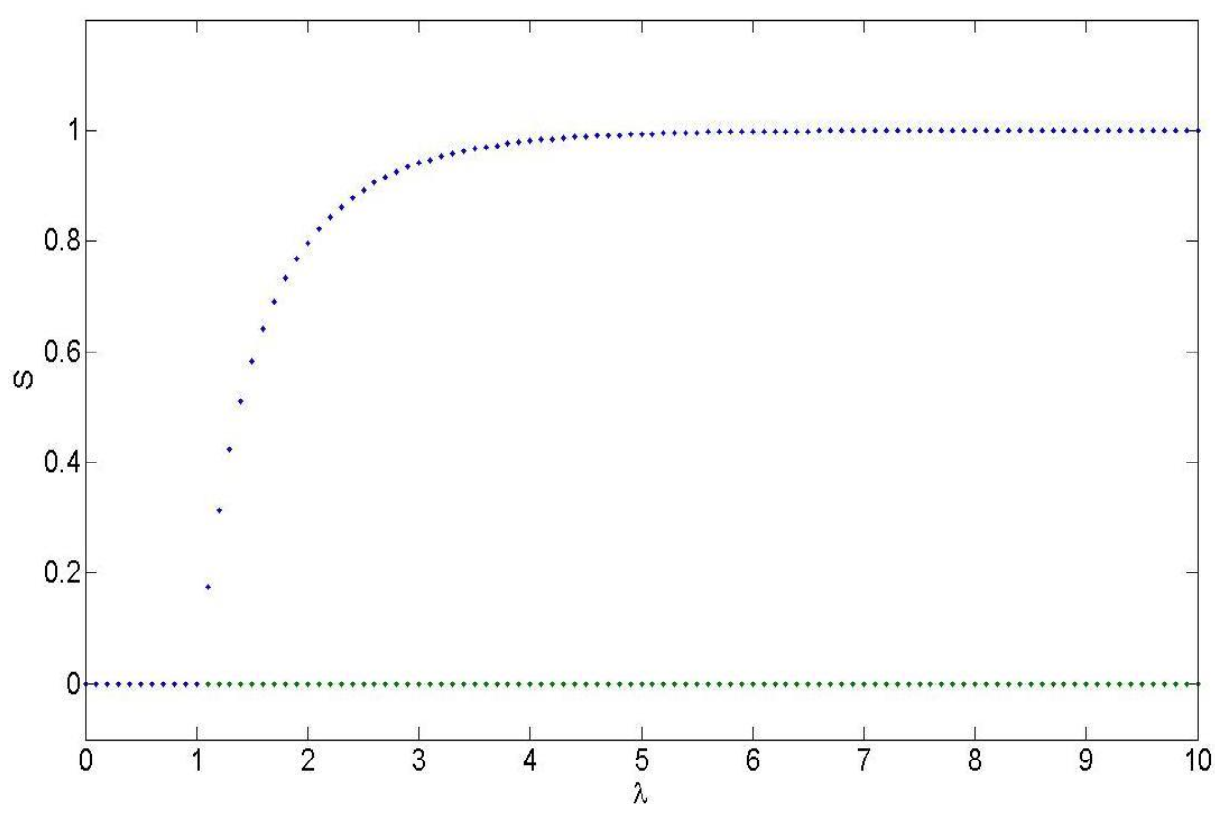
\includegraphics[width=\textwidth]{img/order_parameter_S.png}
    \end{minipage}
\end{figure}

\subsection{Physical Interpretation and the Avalanche Phenomenon}

If the average connectivity slightly exceeds the \(\lambda_c = 1\) threshold (meaning every node has, on average, more than one connection), a path forms such that virtually each node can be reached by any other node in an undirected network. This topological milestone is crucially important for studying the real-world \textbf{spread of diseases, news, or goods} across a network.

\subsubsection{Percolation and Avalanches}
This process shares profound mathematical similarities with the \textbf{percolation model} in physics (the random addition or removal of links from a set of \(N\) nodes).

But \textit{why} is the transition so sudden and explosive (a phase transition)?
Adding links one at a time progressively creates larger and larger distinct clusters. As these clusters grow in size, the statistical probability that a newly added random link will connect \textit{two existing massive clusters} (rather than just attaching to isolated single nodes) increases dramatically.

\begin{figure}[H]
    \begin{minipage}{0.45\textwidth}
        When two large clusters merge, the size of the new combined component jumps discontinuously. This runaway cascading effect of clusters swallowing other clusters is known as the \textbf{"avalanche phenomenon"}, rapidly birthing the Giant Component.

        \caption{The avalanche phenomenon: a new link connecting two existing clusters causes a sudden jump in the size of the giant component.}
    \end{minipage}
    \hfill
    \begin{minipage}{0.5\textwidth}
        \centering
        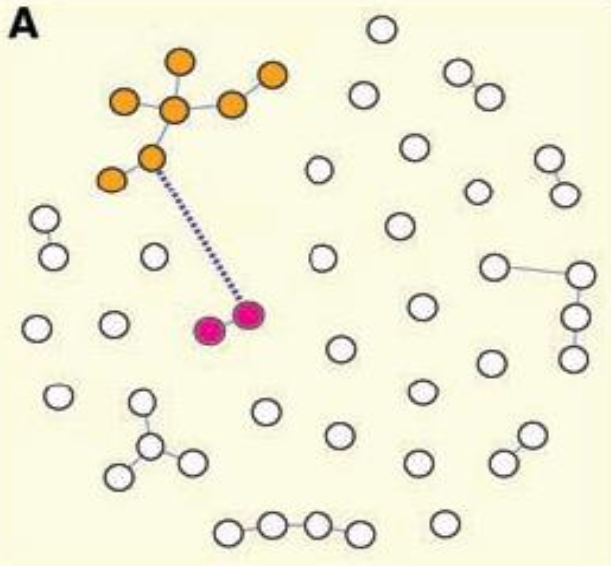
\includegraphics[width=0.9\textwidth]{img/avalanche_phenomenon.png}
    \end{minipage}
\end{figure}

\section{Network Properties in Random Graphs}

We can expect that in a random graph, the properties of the network will be determined by average macroscopic quantities rather than the specific, deterministic configuration of individual nodes and links. By using statistical mechanics approaches, we can understand how complex structural properties naturally arise from the pure random process of connecting nodes.

\subsection{Diameter and Average Path Length}

To estimate the \textbf{diameter} of an Erdős-Rényi (E-R) network, we rely on two fundamental assumptions:
\begin{enumerate}
    \item We consider a sufficiently large \textbf{regular graph} ($N \gg 1$).
    \item The network is \textbf{sparse} ($\#L = O(N)$). This implies the local structure approximates a \textbf{regular tree} (no loops). Because there are no cycles, from any starting node there is a unique path to any other nearby node, and a negligible probability of the path wrapping back to the start.
\end{enumerate}

Starting from a node, one can reach $\langle k \rangle$ nodes in one step. Because we assume a tree-like structure where the degree probabilities $P(k)$ are independent, in two steps one can reach about $\langle k \rangle^2$ nodes, and so on.
After $d$ steps, one can reach approximately $\langle k \rangle^d$ nodes.

To find the diameter (the maximum shortest path), we ask: \textit{In how many steps do we reach all $N$ nodes in the network?}
\[
    \langle k \rangle^d = N
\]
Taking the logarithm of both sides to solve for $d$, we get:
\[
    d = \log_{\langle k \rangle} N = \frac{\ln N}{\ln \langle k \rangle} \implies d \propto \ln N
\]
\textit{(Note on the logarithm base change property used here: $x = b^{\log_b x} = a^{\log_a b \cdot \log_b x} \implies \log_a x = \log_a b \cdot \log_b x$)}.

A mathematically similar result holds for the \textbf{average path length} $\langle l(N) \rangle$ between any two random nodes:
\[
    \langle l(N) \rangle \propto \ln N
\]
As the E-R network size grows, the distance between nodes grows incredibly slowly. To put this into perspective, in a standard regular spatial grid (a D-dimensional lattice), the distance grows much faster as a power of $N$: $N^{1/D}$.

Because of this logarithmic scaling, all purely "random" networks are characterized by highly efficient, easy traversability. This is the statistical origin of the famous \textbf{"small-world" property}. In random graphs, this extreme navigability is actually a "trivial" property. Why? Because the complete absence of \textbf{metric constraints} (physical distances, spatial boundaries, or costs to create long ties) removes the natural bottlenecks that make regular, physical networks less navigable.

\subsection{Degree Correlations}

What relationship exists between the connectivity of two adjacent nodes? In an E-R random graph, there is an \textbf{absence of correlations} between node features. Specifically, there is \textbf{ALMOST none} for finite-size graphs, and strictly \textbf{none in the thermodynamic limit} ($N \gg 1$ and $\#L = O(N)$).

Because links are placed entirely at random without any structural bias, the 2D joint probability of finding an edge connecting a node of degree $k_1$ to a node of degree $k_2$ mathematically breaks down into the simple product of their two independent 1D probabilities:
\[
    p(x_1 = k_1, x_2 = k_2) \approx p(x_1 = k_1) \cdot p(x_2 = k_2)
\]
This mathematical independence makes the E-R graph the perfect \textbf{null model for degree-degree correlation}. If a real-world network exhibits correlation (e.g., high-degree hubs strictly connecting to other high-degree hubs), it definitively proves the network possesses a specific design or evolutionary rule beyond pure randomness.

\subsubsection{In-Degree and Out-Degree Correlations}
Similarly, if we consider an E-R \textbf{directed network}, there is absolutely no correlation between the in-degree ($K_{IN}$) and out-degree ($K_{OUT}$) of the same node:
\[
    p(k_{IN}, k_{OUT}) = p(k_{IN}) \cdot p(k_{OUT})
\]
This means that a node randomly receiving many links (high in-degree) is not statistically more or less likely to project many links (high out-degree).

\begin{figure}[H]
    \begin{minipage}{0.45\textwidth}
        \caption{Scatter plot showing the relationship between in-degree and out-degree in an E-R directed graph. The plot displays a completely uncorrelated, diffuse circular "cloud" of points, visually confirming the total lack of linear dependency between in-degree and out-degree in the E-R model.}
    \end{minipage}
    \hfill
    \begin{minipage}{0.5\textwidth}
        \centering
        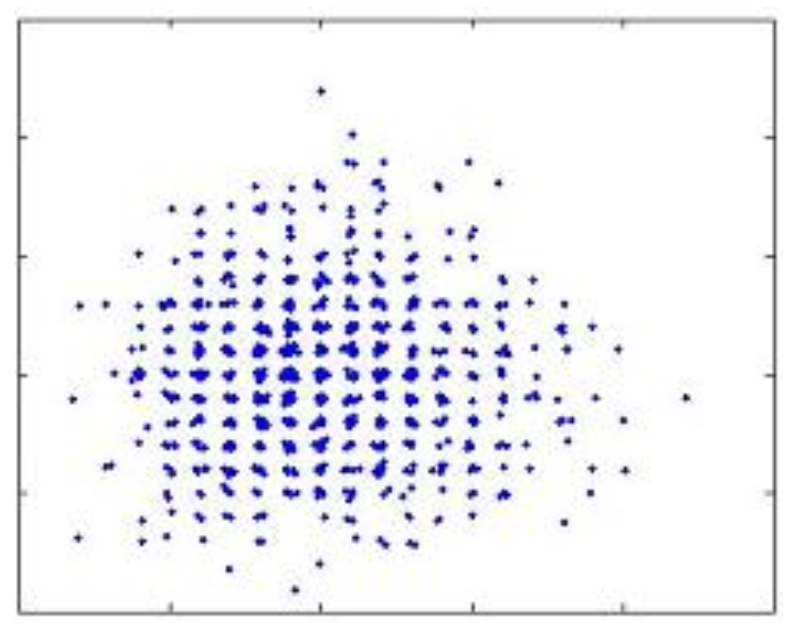
\includegraphics[width=\textwidth]{img/in_out_degree_scatter.png}
    \end{minipage}

\end{figure}

\section{Stochastic Block Model (SBM)}

While the Erdős-Rényi (E-R) model provides a foundational baseline, its strict assumption of a single global connection probability $P$ means it cannot reproduce the localized clustering and modularity observed in real-world systems. To address this limitation, we introduce the \textbf{Stochastic Block Model (SBM)}.

The SBM serves as a \textbf{more complex null model} capable of mathematically modeling non-trivial community structures, while still maintaining the fundamental randomness of the E-R approach within those specific structures.

\subsection{Matrix Construction and Block Probabilities}
The generative process partitions the nodes into distinct groups (communities). The adjacency matrix is then built by combining different E-R sub-matrices:
\begin{itemize}
    \item \textbf{Diagonal Blocks (Intra-community):} These represent connections among nodes within the exact same group. They are generated as standard E-R networks, but typically with a higher specific link density (probability $P_{ii}$). These square blocks can be of different sizes depending on the number of nodes in each community.
    \item \textbf{Non-Diagonal Blocks (Inter-community):} These represent random links connecting nodes from different communities. They are generated with a different probability $P_{ij}$ (usually lower than $P_{ii}$ to simulate separated communities).
\end{itemize}

\textbf{Dimensionality Note:} If we connect a community of size $N$ with a different community of size $M$, the corresponding non-diagonal block of random links in the adjacency matrix will explicitly be \textbf{rectangular}, with dimensions $N \times M$.

From a programming perspective, the main algorithmic backbone remains identical to the one used to generate symmetric or directed E-R networks; it is simply applied piecewise to these specific sub-matrices using their respective densities.

\begin{figure}[H]
    \centering
    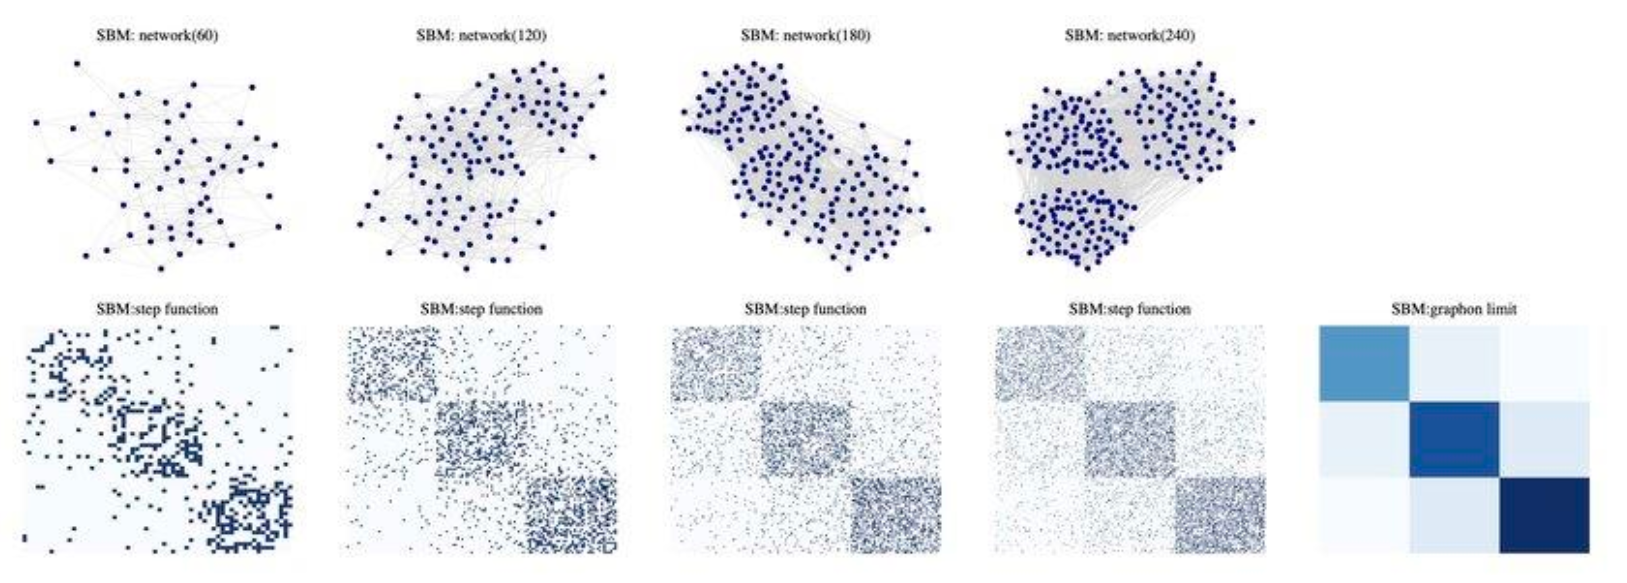
\includegraphics[width=0.8\textwidth]{img/sbm_matrix_construction.png}
    \caption{The construction of the Stochastic Block Model (SBM) adjacency matrix (from 60 to 240 nodes). The matrix is partitioned into diagonal blocks representing intra-community connections (with higher probabilities) and non-diagonal blocks representing inter-community connections (with lower probabilities). The resulting structure allows for the modeling of complex community structures while maintaining the randomness of the E-R model within each block.}
\end{figure}

\subsection{Topological Flexibility of the SBM}
What makes the SBM vastly superior to a simple E-R graph for complex analysis is its parametric flexibility. By simply tweaking the matrix of block probabilities $P_{ij}$, we can generate fundamentally different macroscopic topologies:
\begin{itemize}
    \item \textbf{Assortative Networks:} Diagonal probabilities are strictly greater than non-diagonal ones ($P_{ii} > P_{ij}$). This models standard community structures (like social cliques) where nodes strongly prefer to connect within their own group.
    \item \textbf{Disassortative Networks:} Non-diagonal probabilities are greater than diagonal ones ($P_{ij} > P_{ii}$). Nodes prefer to connect to different groups rather than their own (e.g., bipartite-like structures, or certain biological food webs).
    \item \textbf{Core-Periphery Structure:} One block acts as a dense core with high internal probability, connected to peripheral blocks that have very low internal connection probabilities but rely heavily on ties to the core.
    \item \textbf{Hierarchical Structure:} Blocks can be nested within larger blocks, simulating multiple levels of systemic organization.
\end{itemize}

Ultimately, the SBM is an essential tool because it allows researchers to generate synthetic random networks that explicitly mimic the heterogeneous structural constraints of real-world systems, providing a much more rigorous and realistic statistical baseline for network algorithms.